\section{The CMS Detector}
\label{sec:CMSdetector}

The CMS detector is a general purpose detector installed 100~m underground at the LHC interaction point 5 (P5) near the village of Cessy in France.
It has been designed to exploit the different properties of the wide range of particles and phenomena produced in high-energy collisions in the LHC.
The design of the CMS detector is driven by the challenges of a physics experiment in the LHC environment. 
Many of the physics benchmark channels have a small cross section and the background from QCD jet production is overwhelmingly dominant.
In order to achieve high rejection power with an optimal efficiency for rare channels, the detector has to be able to reconstruct the primary interaction entirely and to reduce the influence of overlapping events. Therefore, one needs to collect all possible information on the particles passing through the detector. Since these have different properties, a mixture of sub-detectors is required for a complete event reconstruction. The reconstruction of lepton signatures is essential for the extraction of rare processes and an excellent muon and electron identification and momentum resolution is desired. A precise measurement of secondary vertices and impact parameters is necessary for an efficient identification of heavy flavor quarks and $\tau$-leptons. Moreover, a large hermetic geometric coverage is preferred, which allows for a precise estimate of the transverse momentum carried away by invisible particles through the sum of all visible particles.

The high peak luminosities of LHC lead to large pileup imposing further challenges to the design. As a consequence of pileup, the products of an interaction under study may be confused with those from other interactions in the same bunch crossing. This effect can be reduced by using high-granularity detectors resulting in low occupancy. In addition, the short bunch crossing requires fast response time and good time resolution of each detector element in order to discriminate the interaction under study from the interactions occurring in neighboring bunch crossings. Hence, a large number of detector channels and an excellent synchronization among them are required. Another challenge arises from the large flux of particles near the interaction point which leads to high radiation levels and the need of radiation hard detectors and front-end electronics.\\

Figure~\ref{fig:CMSlayout} shows the layout of the CMS detector. The detector is built in a cylindrical structure composed of a barrel in the center and endcaps at both sides. This structure is 21.6-m-long, 14.6-m in circumference and 12500-tons-heavy. The detector design and layout was driven by the choice of the magnetic field configuration. Large bending power is needed for a precise measurement of the momentum of high-energy charged particles. Within the CMS detector this is achieved by a superconducting solenoid with a length of 12.9~m and an inner diameter of 5.9~m generating a magnetic field of 4~T. The bore of the magnet coil is large enough to accommodate the inner tracker and the calorimetry inside. 
The inner tracker consists of a pixel and a strip detector both made out of Silicon, and it is the key component of CMS to measure the momenta of charged particles and identify primary and secondary vertices. The calorimetry system comprises a crystal electromagnetic calorimeter (ECAL) and a brass and scintillator hadronic calorimeter (HCAL), which provide information on the energies and directions of all charged and neutral particles. Outside the magnet are the large muon detectors, which, integrated inside the return yokes of the magnet, provide identification of muons and measurement of their momenta.\\

For the description of the CMS detector the following coordinate system is used. The origin is centered at the nominal collision point inside the experiment with the $y$-axis pointing vertically upward, the $x$-axis pointing radially inward toward the center of the LHC, and the $z$-axis points along the beam direction. The azimuthal angle $\phi$ is measured from the $x$-axis in the $x$-$y$ plane. The polar angle $\theta$ is measured from the $z$-axis. Pseudorapidity is defined as $\eta$ = -ln~tan($\theta$/2). Thus, the momentum and energy measured transverse to the beam direction, denoted by \PT and \ET, respectively, are computed from the $x$ and $y$ components.\\

In the following sections the three main components of the CMS detector will be described together with a section on the triggering system.

\begin{figure}[h]
 \begin{center}
  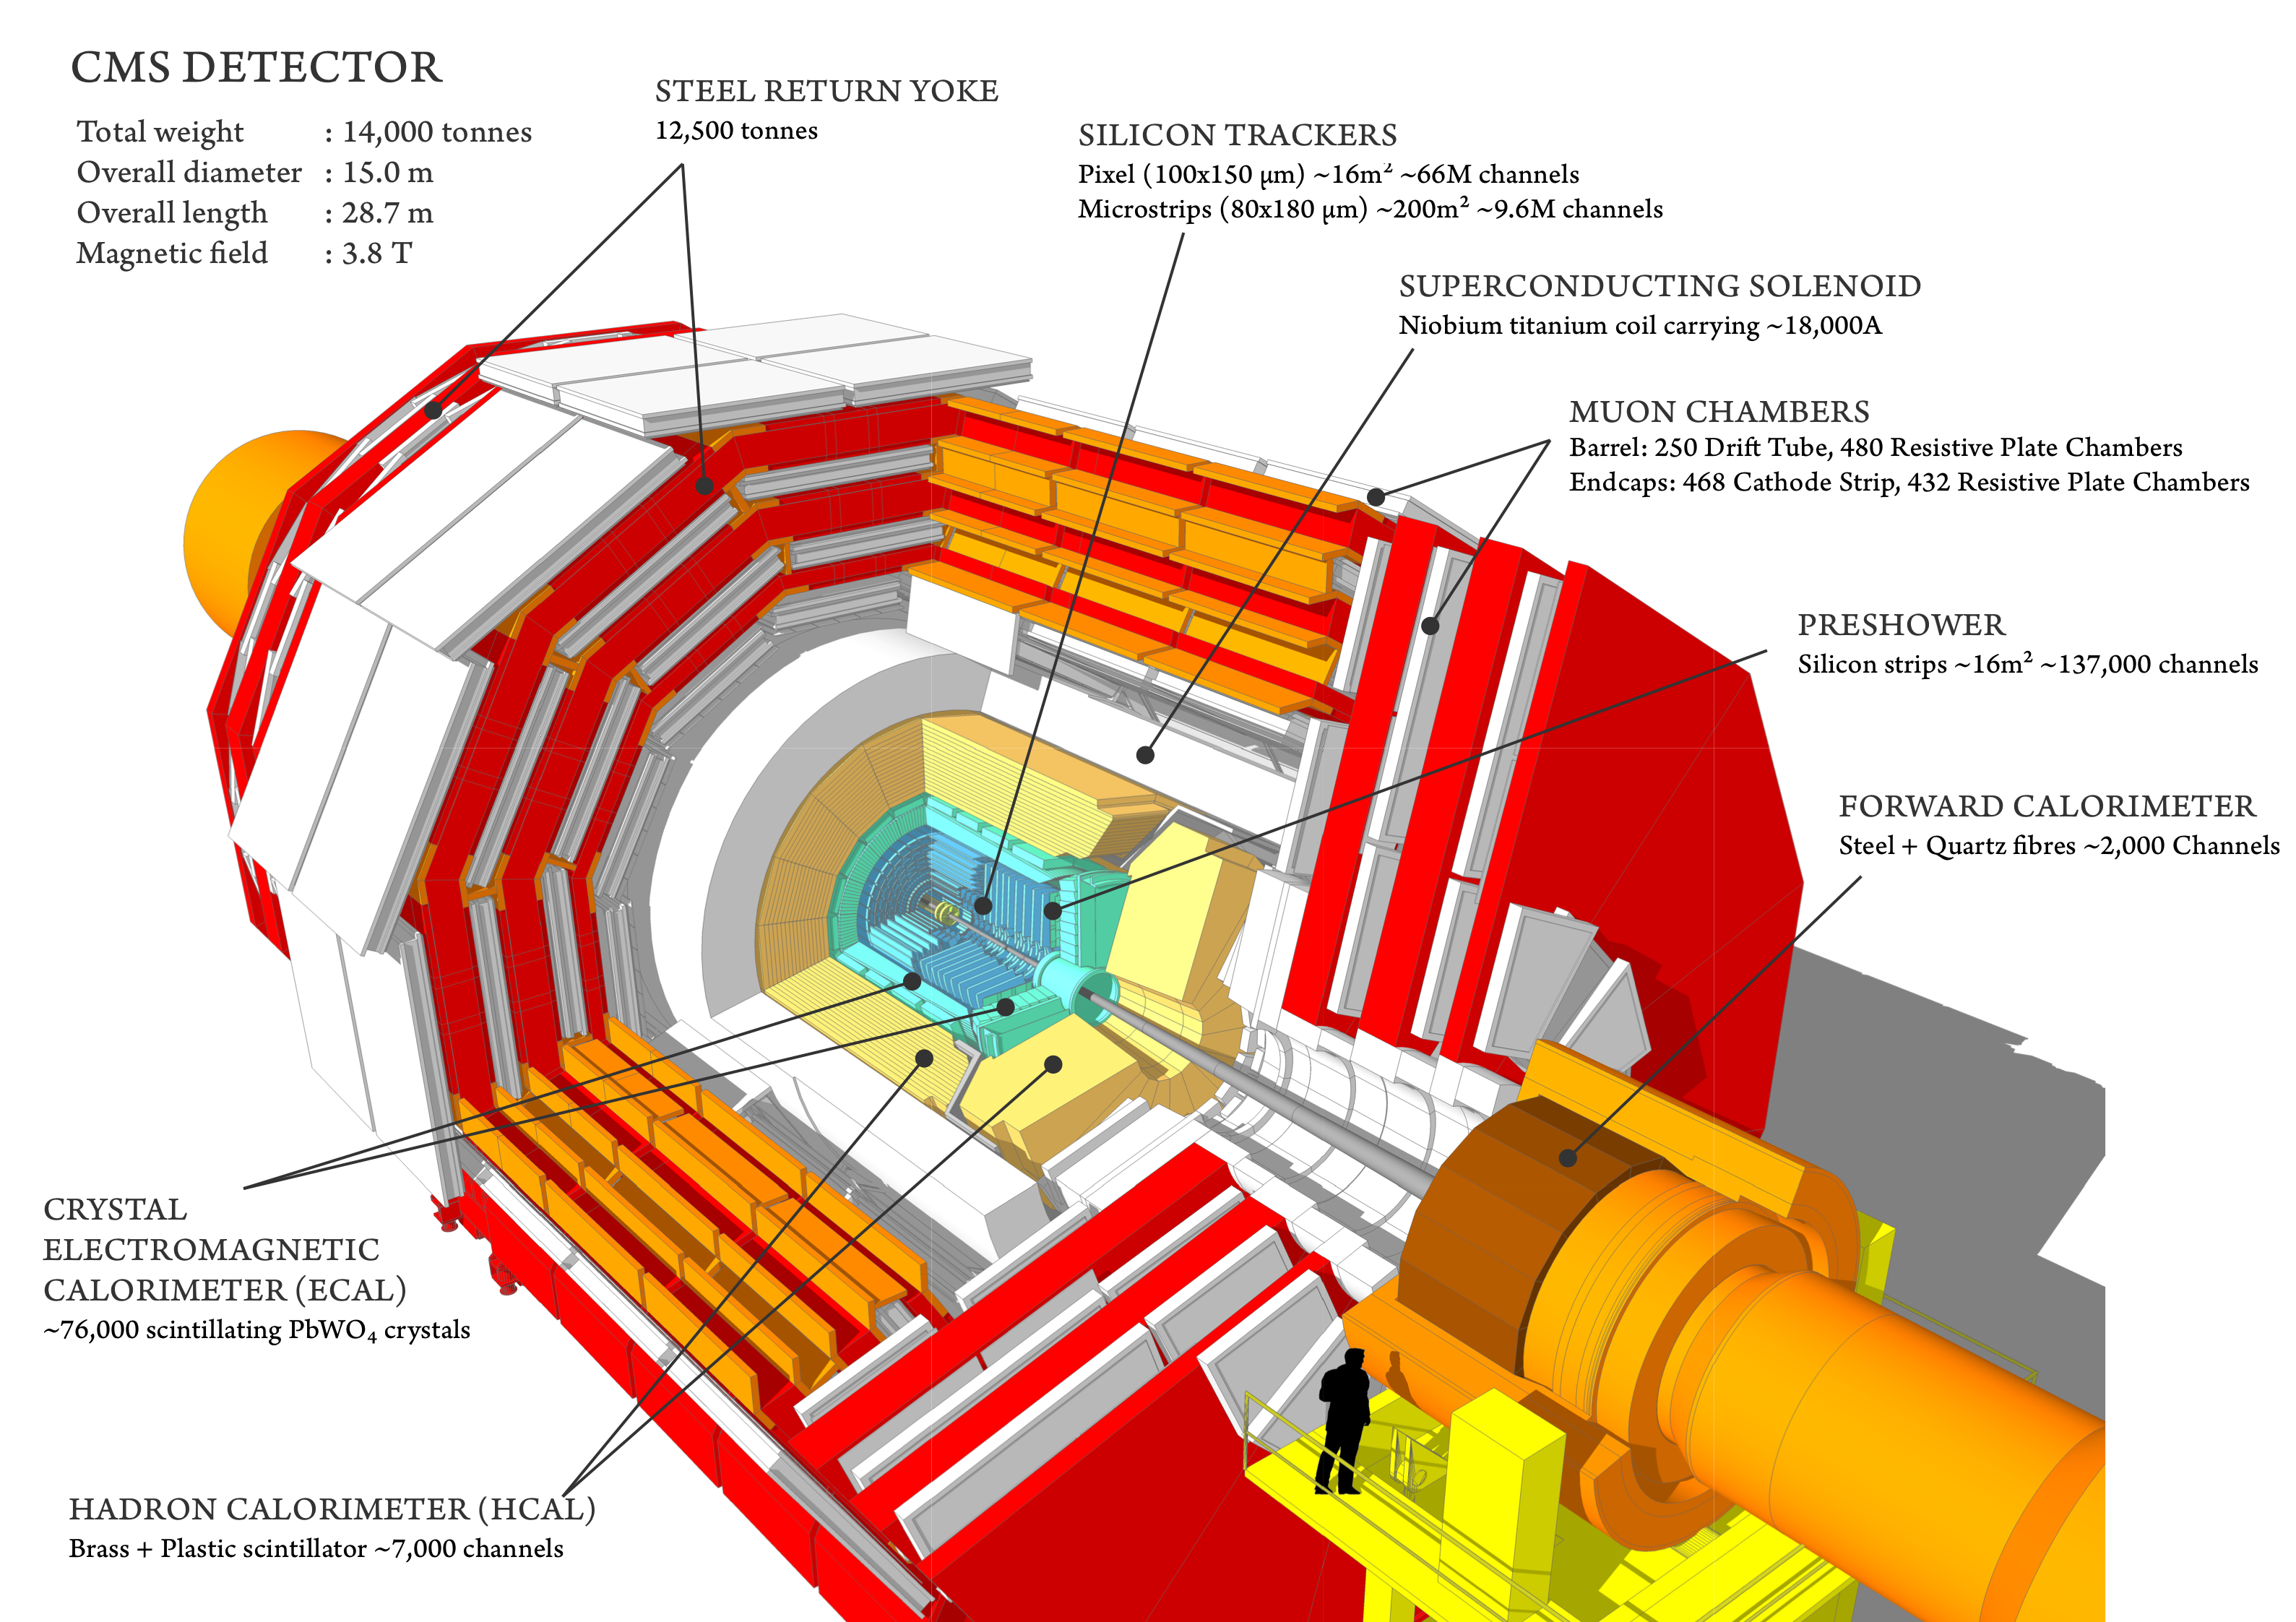
\includegraphics[width=0.9\textwidth]{chapters/Chapter2-CMSatLHC/Figures/cms_120918_03.png}
 \end{center}
 \caption{\small Layout of the CMS experiment and its sub-detectors.}
 \label{fig:CMSlayout}
\end{figure}

\subsection{Tracking detectors}

The tracking system of CMS (Fig.~\ref{fig:TrackerLayout}) is designed to provide a precise and efficient measurement of the trajectories of charged particles emerging from the LHC collisions, as well as a precise reconstruction of secondary vertices~\cite{Karim�ki:368412}. It surrounds the interaction point and has a length of 5.8~m and a diameter of 2.5~m.
In order to achieve high tracking efficiency at the high luminosities of LHC, a detector technology featuring granularity, speed and radiation hardness is required. Furthermore, the material budget of the tracking system has to be as low as possible in order to avoid a worsening of the tracking efficiency and resolution due to material interaction effects of the charged particle, such as multiple scattering, bremsstrahlung, photon conversion or nuclear interactions. These requirements lead to a tracker design entirely based on silicon detector technology. With about 200 m$^2$ of active silicon area the CMS tracker is the largest silicon tracker ever built. It is divided into a pixel detector close to the interaction region and a strip detector in the outer region.
At LHC design luminosity more than 1000 particles are hitting the tracking volume in each bunch crossing. This leads to a hit rate density of 1~MHz/mm$^2$ at a radius of 4~cm which imposes severe challenges to the design of the tracking detectors. With a pixel size of 100$\times$150~$\mu$m$^2$ in $r$-$\phi$ and $z$, respectively, an occupancy of the order of 10$^{-4}$ per pixel and LHC bunch crossing can be achieved. The hit rate density falls with the distance from the interaction point to 60~kHz/mm$^2$ at a radius of 22~cm and to 3~kHz/mm$^2$ at a radius of 115 cm. Therefore, at intermediate radii (20--55~cm), silicon micro-strip detectors are used, with a typical cell length of 10~cm and a pitch of 80~$\mu$m. At the outermost radii (55-110~cm)
the strip size can be further increased to 25~cm$\times$180~$\mu$m. With this choice an occupancy of less than 3\% is maintained in the strip detector.
However, the strip capacitance scales with its length and therefore the electronics noise is a linear function of the strip length as well, becoming not negligible in the outermost region where the strip size is the largest. In order to maintain a good signal to noise ratio of well above 10, CMS uses thicker silicon sensors for the outer tracker region (500~$\mu$m thickness as opposed to the 320~$\mu$m in the inner tracker) with correspondingly higher signal.
%However, the electronic noise scales linearly with the strip capacitance and hence, the length, therefore becoming not negligible in the outermost region where the strip size is the largest.
%Given the large areas that have to be instrumented in this region, also the strip length has to be increased in order to limit the number of read-out channels. 
%However, the strip capacitance scales with its length and therefore the electronics noise is a linear function of the strip length as well. 
To mitigate the radiation damage effects and prolong the lifetime of the detector modules, the tracking detectors are designed to run at subzero temperatures. The cooling is established using a mono-phase liquid cooling system with C$_6$F$_{14}$ as cooling fluid. The whole tracker system operated at +4$^\circ$C during Run 1. After this phase, several improvements have been implemented and an operative temperature of -15$^\circ$C is currently maintained for Run 2.

\begin{figure}[h]
 \begin{center}
  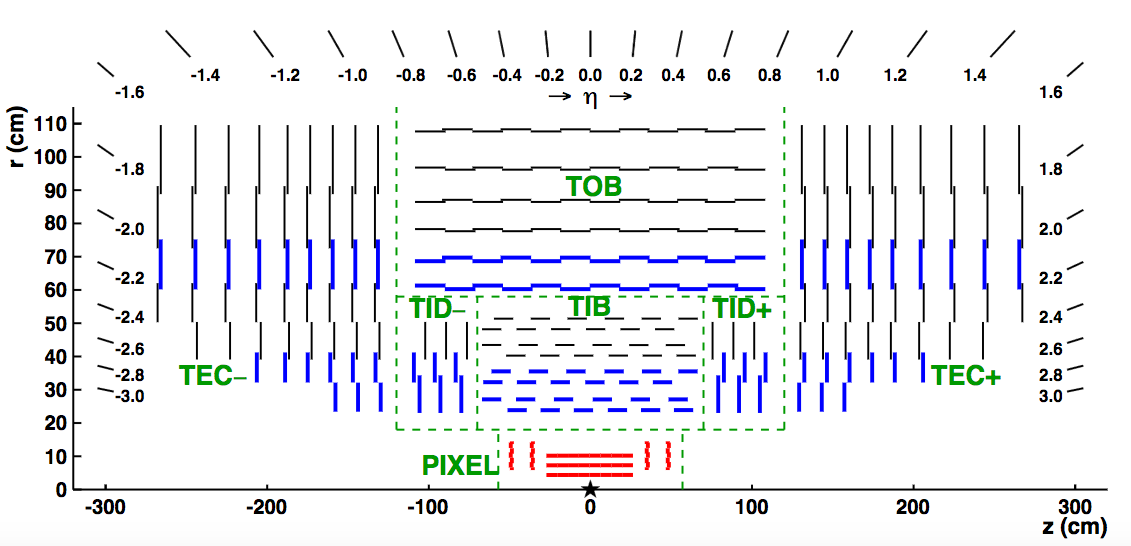
\includegraphics[width=\textwidth]{chapters/Chapter2-CMSatLHC/Figures/tracker.png}
 \end{center}
 \caption{\small Longitudinal section of half of the CMS Tracker system; the different detector types are indicated.}
 \label{fig:TrackerLayout}
\end{figure}



\subsection{The Electromagnetic Calorimeter}
\subsection{The Hadronic Calorimeter}
\subsection{The Muon System}
\subsection{The Trigger System}